En este capítulo se describe el método propuesto para agrupar y reordenar los nodos de un problema de TSP, que consiste en dividir el espacio en cuadrantes dentro de un proceso iterativo.

\subsection{Introducción}
    
Este método de agrupamiento jerárquico recibe un grupo de puntos y lo divide en 4 subgrupos (cuadrantes), cada uno de estos subgrupos en caso de no cumplir con la condición requerida se volverá a dividir en otros 4 subgrupos, y así sucesivamente. Este proceso de división puede repetirse hasta que cada grupo debe tener una cantidad igual o menor al límite establecido previamente.

 \subsection{Aplicación de agrupamiento} 
 
En la figura \ref {fig:FLOWCHART} se puede apreciar un diagrama de flujo cuyos pasos serán explicados con detalle en los siguientes párrafos.\\ 

\begin{figure}[hbtp]
   \centering
   \begin{tikzpicture}[node distance=1.5cm]

        \node (start) [startstop] 
		{
			\small	Inicio
		};
        \node (in1) [io, below of=start,] 
		{
        	\small	Recibe una lista de puntos
        };
        \node (dec1) [decision, below of=in1,yshift=-1.5cm] 
		{
        	\small	¿La lista mencionada supera el límite?
        };
        \node (pro1) [process, below of=dec1, yshift=-1.5cm] 
		{
        	\small	Dividir los puntos en 4 cuadrantes
        };
        \node (pro1_1) [process, below of=pro1, yshift=-0.1cm] 
		{
        	\small	Reordenar los cuadrantes
        };
        \node (pro1_2) [process, below of=pro1_1, yshift=-0.1cm] 
		{
        	\small	Tomar el siguiente cuadrante de la lista y comprobar
        };
        \node (pro2) [process, right of=dec1, xshift=7cm] 
		{
        	\small	Resolver mediante fuerza bruta
        };
        \node (pro2_1) [process, below of=pro2, yshift=-0.1cm] 
		{
        	\small	Agregar lista ordenada a la solución
        };
        \node (dec2) [decision, below of=pro2_1, yshift=-3cm] 
		{
        	\small	¿Quedan mas cuadrantes?
        };
        \node (pro3_1) [process, below of=dec2, yshift=-1.5cm] 
		{
        	\small	Mostrar los puntos que conforman la solución
        };
        \node (Fin) [startstop, below of=pro3_1, yshift=-0.1cm] 
		{
			\small	Fin
		};
        
        \draw [arrow] (start) -- (in1);
        \draw [arrow] (in1) -- (dec1);
        \draw [arrow] (dec1) -- node[anchor=east] {SI} (pro1);
        \draw [arrow] (pro1) -- (pro1_1);
        \draw [arrow] (pro1_1) -- (pro1_2);  
        \draw [arrow] (pro1_2.west) -- ([xshift=-2cm]pro1_2.west) |- (dec1);    
        \draw [arrow] (dec1) -- node[anchor=south] {NO} (pro2);
        \draw [arrow] (pro2) -- (pro2_1);
        \draw [arrow] (pro2_1) -- (dec2);
        \draw [arrow] (dec2) -- node[anchor=south] {SI} (pro1_2);
        \draw [arrow] (dec2) -- node[anchor=east] {NO} (pro3_1);
        \draw [arrow] (pro3_1) -- (Fin);
		
    \end{tikzpicture}       
    \caption{Diagrama de flujo del método de cuadrantes.}
    \label{fig:FLOWCHART}
\end{figure} 

\hspace*{1cm} Como indica la figura \ref {fig:FLOWCHART} después de recibir una lista de puntos y que su tamaño supere el límite establecido se dividirá en 4 cuadrantes de un plano cartesiano; una vez distribuidos se comprobará cada cuadrante para determinar si supera el límite. Cada cuadrante se dividirá en 4 de manera recursiva.\\
\hspace*{1cm} Si en algún momento del proceso la lista de puntos a comprobar no supera el límite se procederá a resolver mediante un proceso de fuerza bruta buscando la secuencia de puntos que produzca la ruta más corta; ya con estos puntos reordenados se agregarán a una nueva lista que representará la solución del problema, estos al leerse en ese orden mostrará la ruta a recorrer.\\
\hspace*{1cm} Ahora ya con este diagrama explicado se necesita determinar la forma en que el algoritmo determina hacia que cuadrante irá cada punto, para ello se tendrá que crear un punto adicional que servirá de centro. Para calcular el centro es necesario tomar como base la coordenada del punto más lejano tanto a la izquierda como a la derecha para el eje X´ y el más lejano de arriba hacia abajo para hacer el eje Y´; una vez que se encuentre un subgrupo que satisfaga el criterio se colocará el cursor (el supuesto agente viajero) e iniciará a recorrer el cuadrante. La figura \ref {fig:rectangulo} muestra un ejemplo de la definición del centro.\\
\hspace*{1cm} En la figura \ref {fig:rectangulo} se observa que el punto 5 es el que se encuentra más alejado a la izquierda y el 4 más alejado a la derecha, así como los puntos 2 y 4 de abajo hacia arriba respectivamente, por tanto el centro es el punto medio entre el ancho y alto de ambos.\\
\hspace*{1cm} El siguiente proceso consiste en buscar la mejor combinación que exista para llegar desde el punto donde está iniciando el recorrido al siguiente cuadrante. Para lograr este objetivo se usarán unos puntos creados para la ocasión que son intersecciones de un cuadrante a otro, estos servirán para indicar la salida y entrada de los cuadrantes.\\
\hspace*{1cm} Como se explicó anteriormente estos cuadrantes creados a partir de estos agrupamientos se unirán de cuadrante a cuadrante hasta que se recorran todos; al final del problema todos los puntos se encontrarán conectados. Todos los cuadrantes ya resueltos se unirán, de preferencia con el cuadrante que tenga adyacente y cuando los 4 subcuadrantes del cuadrante se hayan unido, se buscará otro cuadrante adjunto y así sucesivamente, el proceso terminará hasta resolver todos los cuadrantes.\\
 \begin{figure}[hbtp]
    \centering
        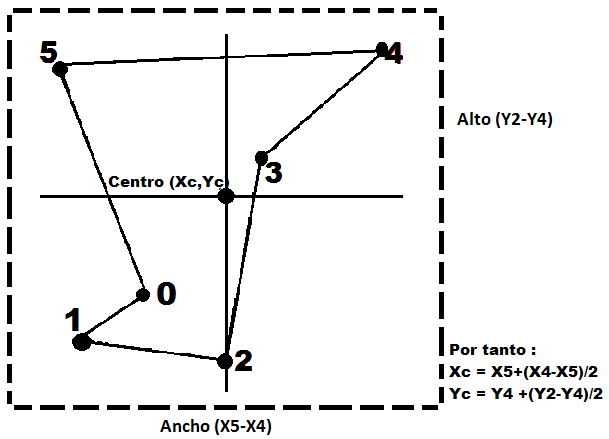
\includegraphics[width=0.95\textwidth]{MetodoRectanguloAureo/Imagenes/rectangulo.png}
        \caption{Ejemplo para calcular el centro del plano de búsqueda.}
        \label{fig:rectangulo}
\end{figure}

%\clearpage \newpage
%\begin{lstlisting}[language=JAVA, caption=Algoritmo Base del Método de Cuadrantes, label=lst:codigo11,escapechar=|]
funcion Inicio()
 {
	RutaSolucion{Puntos[n]}
	ArregloCuadrantes{Cuadrantes[Puntos[n]]}
	Limite = n
	Direccion = derecha
	SubcuadranteOrigen = -1
	CuadranteOrigen = -1
	CuadranteDestino = -1
	Comprobar()
}
funcion Comprobar()
{
	 While (ArregloCuadrantes.length > 0)
	 {
		CuadrantesActual = ArregloCuadrantes[0]
		l = 0
		While CuadrantesActual.length < l {
			PuntosActual = CuadrantesActual[l]
			If(PuntosActual.length < Limite)
			{
				Resolver()
			} 
			else 
			{
				Dividir()  
			}
			l++
		} 
		ArregloCuadrantes.remover[0]
	}
	Terminar()
}	
funcion Dividir()
{
	NuevosCuadrantes{Cuadrantes[Puntos[n]],Cuadrantes[Puntos[n]],Cuadrantes[Puntos[n]],Cuadrantes[Puntos[n]]} = Dividir PuntosActual en 4
	Se reordena el orden de los elementos de NuevosCuadrantes de acuerdo al automata de cuadrantes de la figura \ref {fig:automata.png}
		  -Para ello se calculan 2 ejes (X y Y) a partir de los valores que forman los puntos de ese cuadrante, de ahi se establece el centro que es igual a los valores divididos en 2
		  - A partir de ahi se establece el orden de cuadrantes que va a recorrer para completar la ruta basandose en
				-SubcuadranteOrigen: El cuadrante donde se encuentra
				-En caso de que el cuadrante pertenezca a uno mas grande, el cuadrante al que planea dirigirse el cuadrante padre
					-En caso de no ser menor a 0 significa que planea regresar a si mismo, por tanto puede viajar a direccion, izquierda,derecha,arriba o abajo (por preferencia se eligio izquierda), en el automata de la figura |\ref {fig:automata.png}| se interpretara como estado |$\lambda$|                    
				-En caso de que el cuadrante pertenezca a uno mas grande, el numero de cuadrante padre al que pertenece
					-En caso de no ser menor a 0 significa que planea regresar a si mismo, por tanto puede viajar a dirección, izquierda,derecha,arriba o abajo (por preferencia se eligio izquierda), en el automata de la figura |\ref {fig:automata.png}| se interpretara como estado |$\lambda$|       
	Agregar NuevosCuadrantes a ArregloCuadrantes reemplazando PuntosActual en el mismo lugar donde estaban
	Comprobar()	
}
funcion Resolver()
{
	PuntosActual = Reordenar orden de los elementos de PuntosActual usando metodo de Fuerza Bruta probando todas las combinaciones posibles y obtener el mejor resultado
	agregar PuntosActual a RutaSolucion
	Comprobar()
}
function Terminar()
{
	Mostrar resultados de RutaSolucion
}	
\end{lstlisting}   

\hspace*{1cm} El siguiente paso es definir el criterio que se aplica para saber en qué orden de subcuadrantes debe viajar para recorrer toda la sección.

\subsection{Aplicación de autómatas para el orden de los cuadrantes} 

Para determinar el orden de los cuadrantes por recorrer se utilizará un autómata que recibirá ciertos parámetros y devolverá una de varias soluciones predeterminadas. Los 3 parámetros del autómata son:
    \begin{itemize}
        \item El cuadrante origen: El cuadrante donde se encuentra el cursor.
        \item El cuadrante destino: El cuadrante a donde se dirigirá el cursor.
        \item El origen del subcuadrante: El subcuadrante del cuadrante origen de donde inicia la ruta.
    \end{itemize}
     \begin{figure}[hbtp]
        \centering
            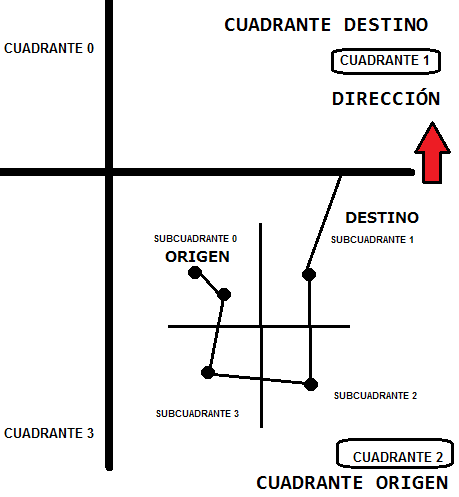
\includegraphics[width=0.6\textwidth]{MetodoRectanguloAureo/Imagenes/findpriori.png}
            \caption{Fragmento de ejemplo del método de cuadrantes.}
            \label{fig:findpriori.png}
    \end{figure}
\hspace*{1cm} En la figura \ref {fig:findpriori.png} se puede observar el fragmento de un ejemplo donde se presentan los cuadrantes 1 y 2; dentro del cuadrante 2 se puede observar que también está dividido en otros subcuadrantes y el punto de origen se encuentra en el subcuadrante 0; de esta forma se obtienen los parámetros necesarios donde:
    \begin{itemize}
        \item El cuadrante origen es 2.
        \item El cuadrante destino es 1.
        \item El origen del subcuadrante es 0.
    \end{itemize}
\hspace*{1cm} Lo primero a notar es que el cursor tendrá que viajar hacia arriba recorriendo los 4 cuadrantes sin pasar por el anterior ya que el cuadrante destino está sobre el cuadrante origen. Para ello se hará uso de una matriz de direcciones presentada en la figura \ref {fig:automatchart.png}.\\

     \begin{figure}[hbtp]
        \centering
            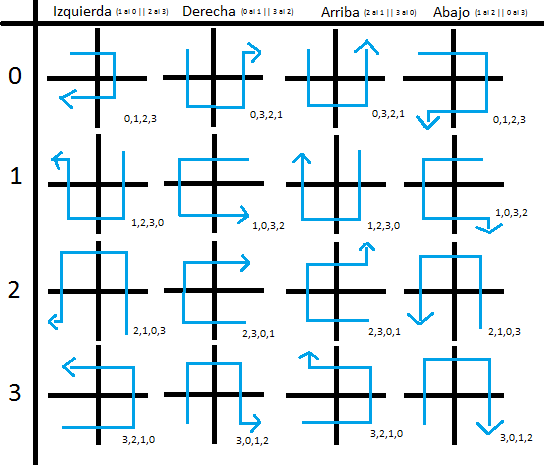
\includegraphics[width=0.8\textwidth]{MetodoRectanguloAureo/Imagenes/automatchart.png}
            \caption{Matriz de direcciones.}
            \label{fig:automatchart.png}
    \end{figure}
    
\hspace*{1cm} Como se puede ver en la figura \ref {fig:automatchart.png} ésta es una matriz de 4 filas y 4 columnas, las filas representan el origen del subcuadrante en donde se va a empezar  (en este caso 0) y las columnas representan la dirección a la que tiene que ir (en este caso hacia arriba y del cuadrante 2 al 1), al tener estas 2 coordenadas se determina como solución la secuencia (0,3,2,1) que determina el orden de subcuadrantes por los que tiene que viajar para pasar por todos los puntos. Cada subcuadrante puede seguir dividiéndose, para tal caso el subcuadrante del origen es siempre el que se está resolviendo al momento, el cuadrante origen y cuadrante destino forman parte del cuadrante anterior.\\
\hspace*{1cm} La primera vez que se vaya a dividir el conjunto de puntos, el parámetro de destino será el mismo punto de origen por tanto; ya teniendo los otros 2 parámetros se puede tomar la solución de cualquiera de las 4 columnas, dando 4 posibles soluciones dependiendo del giro principal. En la figura \ref {fig:example.png} se podrá ver un ejemplo completo aplicando todas las reglas mencionadas.\\

     \begin{figure}[hbt]
        \centering
            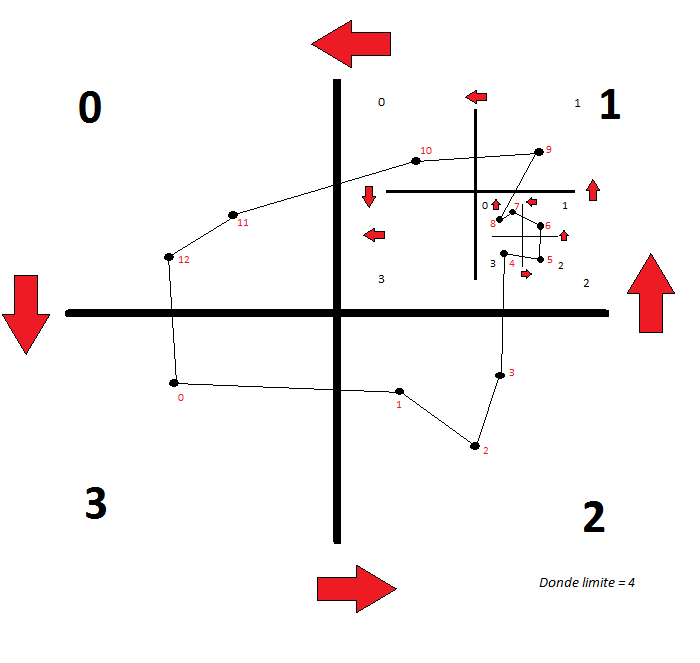
\includegraphics[width=0.7\textwidth]{MetodoRectanguloAureo/Imagenes/example.png}
            \caption{Ejemplo completo de un problema TSP aplicando las reglas mencionadas.}
            \label{fig:example.png}
    \end{figure}
    
\subsubsection{Descripción del autómata}    

En la figura \ref {fig:automata.png} se puede ver el autómata que recibe los 3 parámetros (el cuadrante inicial, el cuadrante donde se tiene que dirigir, y por último el origen del subcuadrante). En la tabla \ref{table:DeclaracionAutomata} se podrá ver su declaración formal.\\

    \begin{figure}[hbtp]
        \centering
            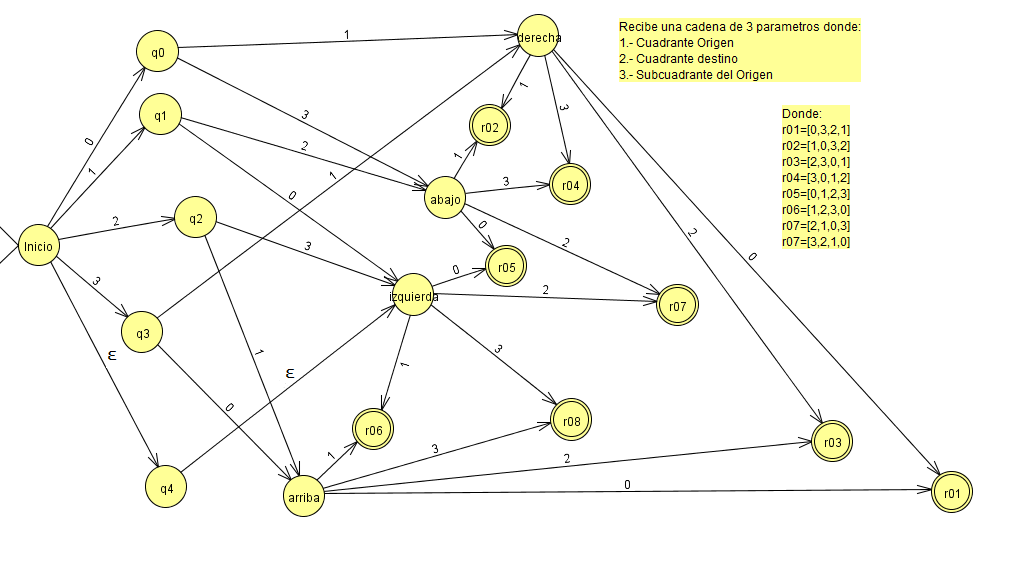
\includegraphics[width=1\textwidth]{MetodoRectanguloAureo/Imagenes/automata2_b.png}
            \caption{Autómata del método de cuadrantes.}
            \label{fig:automata.png}
    \end{figure}    

    \begin{table}[hbtp]
		\centering
		   \caption{Elementos del autómata del método de cuadrantes.}		
		   \begin{tabular}{ | l | l |}
		   \hline
			\rowcolor[gray]{0.5}
			 \hline\multicolumn{2}{|c|}{ \rowcolor[gray]{0.5}Declaración formal} \\\hline
		   \textbf{$\Sigma$}:  & 0, 1, 2, 3      \\ \hline
				 \textbf{$Q$}: & Inicio, q0, q1, q2, q3,q4\\   
							   & izquierda, derecha, arriba, abajo,\\ 
							   & r01, r02, r03, r04, r05, r06, r07, r08     \\ \hline
				\textbf{$q0$}: & Inicio     \\ \hline
				\textbf{$F$}:  & r01, r02, r03, r04, r05, r06, r07, r08     \\ \hline
			\textbf{$\delta$}: & Es la relación de transiciones que se muestran en la tabla \ref{table:Automata}. \\ \hline
		   \end{tabular}
		   \label{table:DeclaracionAutomata}
       \end{table}
       
\hspace*{1cm} Como se puede ver en la tabla \ref{table:Automata}, la transición de eventos que realiza el autómata es del tipo no determinista ya que posee estados vacíos y transiciones $\epsilon$.

	 \begin{table}[hbtp]
		 \centering
			\caption{Transiciones del autómata del método de cuadrantes.}		 
			\begin{tabular}{ | l | l | l | l | l | l |}
			\hline
			  \rowcolor[gray]{0.5}
				   & 0         & 1       & 2       & 3         &$\epsilon$   \\ \hline
			Inicio & q0        & q1      & q2      & q3        & q4         \\ \hline      
				q0 &           & derecha &         & abajo     &            \\ \hline
				q1 & izquierda &         & abajo   &           &            \\ \hline
				q2 &           & arriba  &         & izquierda &            \\ \hline
				q3 & arriba    &         & derecha &           &            \\ \hline
				q4 &           &         &         &           & izquierda  \\ \hline
		 izquierda & r05       & r06     & r07     & r08       &            \\ \hline
		   derecha & r01       & r02     & r03     & r04       &            \\ \hline
			arriba & r01       & r06     & r03     & r08       &            \\ \hline
			 abajo & r05       & r02     & r07     & r04       &            \\ \hline
			  *r01 &           &         &         &           &            \\ \hline
			  *r02 &           &         &         &           &            \\ \hline
			  *r03 &           &         &         &           &            \\ \hline
			  *r04 &           &         &         &           &            \\ \hline
			  *r05 &           &         &         &           &            \\ \hline
			  *r06 &           &         &         &           &            \\ \hline
			  *r07 &           &         &         &           &            \\ \hline
			  *r08 &           &         &         &           &            \\ \hline
			\end{tabular}
			\label{table:Automata}
	\end{table}
    

    
\hspace*{1cm} En el ejemplo a la figura \ref {fig:example.png} el cuadrante 1 está dividido en otros subcuadrantes, el origen del subcuadrante sería el punto el 4 que se encuentra en el cuadrante 2, ya que a la dirección por la que va tiene que ir al cuadrante principal 0. Por tanto, los parámetros que recibiría el autómata en ese mismo orden sería: 

\begin{itemize}
\item El cuadrante origen: El cuadrante 1.
\item El cuadrante destino:El cuadrante 0 que se encuentra a su izquierda.
\item El origen del subcuadrante: El subcuadrante 2.
\end{itemize}

\hspace*{1cm}Como se observa en la figura \ref {fig:automata.png}, primero se recorrería al estado $q2$, luego pasaría por el estado $izquierda$ y por último al estado $r7$, dando como resultado los parámetros (2,1,0,3) que vendrían siendo los cuadrantes por recorrer en la iteración inicial. Sin embargo el subcuadrante 1 excede con el límite de puntos establecido teniendo que resolver primero este inconveniente repitiendo el proceso de subdivisión esta vez poniendo el origen, destino y subcuadrante del origen como 2, 1 y 3 respectivamente, lo que daría el estado $r8$ con los parámetros (3,2,1,0).\\
\hspace*{1cm} De ahí en adelante se resuelven los demás cuadrantes usando el método de fuerza bruta, que gracias a las divisiones que se fueron haciendo agilizan el proceso, terminando mucho más rápido que haber intentado hacer el método de fuerza bruta con todos los puntos.\\

\subsection{Comentarios finales}
Este método hace uso del sentido común y de la distribución uniforme para cumplir con el objetivo deseado, no se busca obtener todavía un resultado definitivo, sino una buena solución que servirá de base para la aplicación de las metaheurísticas correspondientes.\\
\hspace*{1cm} El uso de cuadrantes permite seccionar por zonas de manera finita y no salir de cada una de ellas hasta pasar por todos los lugares, reduciendo el tiempo de cálculo y evitando realizar combinaciones innecesarias.\\ 
\hspace*{1cm} Sin embargo y a pesar de obtener una buena solución, el resultado obtenido a través de este algoritmo no es la mejor ruta que se haya creado hasta la fecha, sino es una respuesta cercana que se puede refinar aplicando metaheurísticas, tema que se verá en el capítulo 5.\\
\hspace*{1cm} Lo que destaca de este método es la de obtener buenos resultados y la preferencia de recorrer zonas cercanas con tiempos de cálculo breves en lugar de intentar hacer movimientos audaces o combinaciones reiterativas que pueden ser solo una pérdida de tiempo, aunque eso también implica una desventaja ya que jamás podría obtener resultados mejores a costa de mayor trabajo.\\
\hspace*{1cm} Como se muestra en la figura \ref {fig:monalisatsp2.png}, es un retrato de la Mona Lisa hecho a base de un problema de TSPLIB obtenido de \cite{[MONALISA]}, usando el algoritmo de cuadrantes se pudo unir los puntos que componían el problema mostrando la figura presentada.
    \begin{figure}[hbtp]
        \centering
            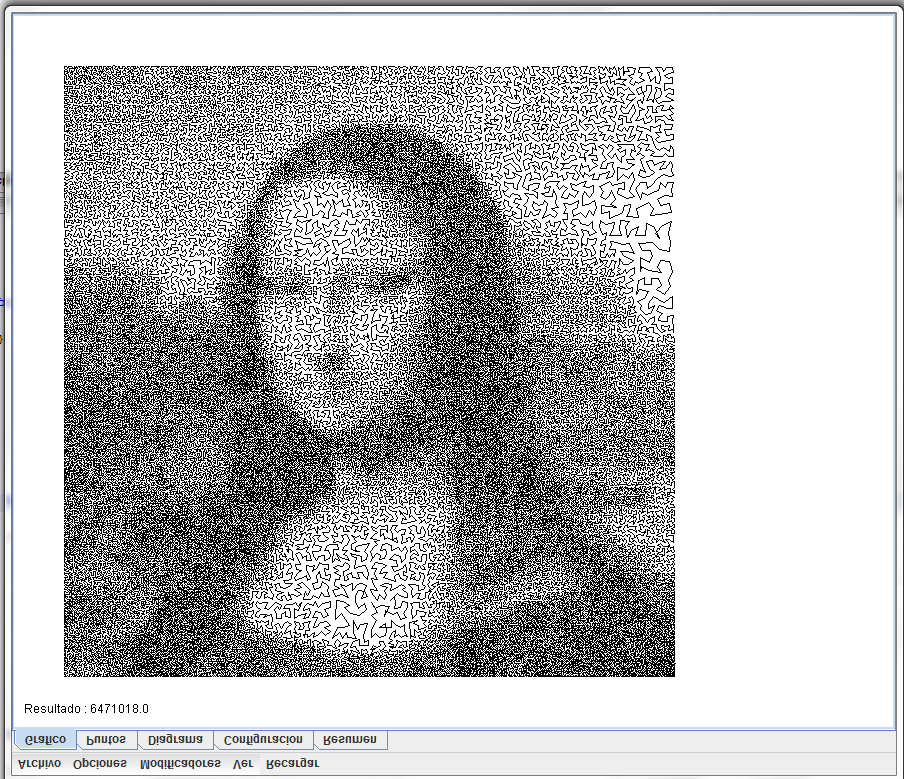
\includegraphics[width=0.9\textwidth]{MetodoRectanguloAureo/Imagenes/monalisatsp.png}
            \caption{Ejemplo de ejercicio de la MonaLisa hecha en TSP.}
            \label{fig:monalisatsp2.png}
    \end{figure}